\documentclass[]{article}
\usepackage{lmodern}
\usepackage{amssymb,amsmath}
\usepackage{ifxetex,ifluatex}
\usepackage{fixltx2e} % provides \textsubscript
\ifnum 0\ifxetex 1\fi\ifluatex 1\fi=0 % if pdftex
  \usepackage[T1]{fontenc}
  \usepackage[utf8]{inputenc}
\else % if luatex or xelatex
  \ifxetex
    \usepackage{mathspec}
  \else
    \usepackage{fontspec}
  \fi
  \defaultfontfeatures{Ligatures=TeX,Scale=MatchLowercase}
\fi
% use upquote if available, for straight quotes in verbatim environments
\IfFileExists{upquote.sty}{\usepackage{upquote}}{}
% use microtype if available
\IfFileExists{microtype.sty}{%
\usepackage{microtype}
\UseMicrotypeSet[protrusion]{basicmath} % disable protrusion for tt fonts
}{}
\usepackage[margin=1in]{geometry}
\usepackage{hyperref}
\hypersetup{unicode=true,
            pdftitle={Testosterone, diversity, and group project performance},
            pdfauthor={Cathy Su},
            pdfborder={0 0 0},
            breaklinks=true}
\urlstyle{same}  % don't use monospace font for urls
\usepackage{longtable,booktabs}
\usepackage{graphicx,grffile}
\makeatletter
\def\maxwidth{\ifdim\Gin@nat@width>\linewidth\linewidth\else\Gin@nat@width\fi}
\def\maxheight{\ifdim\Gin@nat@height>\textheight\textheight\else\Gin@nat@height\fi}
\makeatother
% Scale images if necessary, so that they will not overflow the page
% margins by default, and it is still possible to overwrite the defaults
% using explicit options in \includegraphics[width, height, ...]{}
\setkeys{Gin}{width=\maxwidth,height=\maxheight,keepaspectratio}
\IfFileExists{parskip.sty}{%
\usepackage{parskip}
}{% else
\setlength{\parindent}{0pt}
\setlength{\parskip}{6pt plus 2pt minus 1pt}
}
\setlength{\emergencystretch}{3em}  % prevent overfull lines
\providecommand{\tightlist}{%
  \setlength{\itemsep}{0pt}\setlength{\parskip}{0pt}}
\setcounter{secnumdepth}{0}
% Redefines (sub)paragraphs to behave more like sections
\ifx\paragraph\undefined\else
\let\oldparagraph\paragraph
\renewcommand{\paragraph}[1]{\oldparagraph{#1}\mbox{}}
\fi
\ifx\subparagraph\undefined\else
\let\oldsubparagraph\subparagraph
\renewcommand{\subparagraph}[1]{\oldsubparagraph{#1}\mbox{}}
\fi

%%% Use protect on footnotes to avoid problems with footnotes in titles
\let\rmarkdownfootnote\footnote%
\def\footnote{\protect\rmarkdownfootnote}

%%% Change title format to be more compact
\usepackage{titling}

% Create subtitle command for use in maketitle
\providecommand{\subtitle}[1]{
  \posttitle{
    \begin{center}\large#1\end{center}
    }
}

\setlength{\droptitle}{-2em}

  \title{Testosterone, diversity, and group project performance}
    \pretitle{\vspace{\droptitle}\centering\huge}
  \posttitle{\par}
    \author{Cathy Su}
    \preauthor{\centering\large\emph}
  \postauthor{\par}
      \predate{\centering\large\emph}
  \postdate{\par}
    \date{9/10/2019}


\begin{document}
\maketitle

\hypertarget{executive-summary}{%
\subsection{Executive Summary}\label{executive-summary}}

In this report, we analyzed a demographic data set collected by
\emph{(Akinola et al. 2018)} and explore the relationship between a set
of variables that contribute to group performance on a competetive task.
The data comprises individual level and group level statistics collected
from groups of MBA students completing a 7-day group project. We use
exploratory data analysis and regression models to mainly explore how
\textbf{diversity, cortisol and testosterone} levels affect
\textbf{final.performance}. The f-test shows that diversity score,
cortisol and testosterone individually do not significantly affect
final.performance.

Then, we fit several linear regression models and found that the model
with the highest adjusted R squared value predicts performance as a
function of average log testosterone, diversity and group size. In this
model, if we hold group size constant, indeed diversity has a positive
effect on performance, but only if group-level testosterone is low.

\hypertarget{introduction}{%
\subsection{Introduction}\label{introduction}}

Diversity and conflict are considered important factors which influence
how well we work in groups (Knippenberg and Schippers 2007). As the
working world becomes more connected across the globe and thus the
diversity of organizational groups increases, it is important to
characterize the effect of diversity on group performance. Previous work
by (Akinola et al. 2018) suggests that both diversity and group hormone
levels will influence how well groups perform on a competetive task. In
their study, they considered levels of the two hormones testosterone and
cortisol. Testosterone is involved in dominance and competition related
behaviour in individuals and is produced at a higher level in males than
females, while cortisol is a hormone released during physical and
psychological stress (Mehta and Prasad 2015). For healthy males between
19 to 40 years, normal testosterone is known to fall within the 15.4 to
13 nmol/L range (Kelsey et al. 2014). Healthy levels of hormones for men
and women are given in Table, collected from (Matsuzaka et al. 2013)

In their work, (Akinola et al. 2018) collected both demographic data and
hormone measurements from 370 MBA students organized into 74 groups who
partcipated in a competitive week long project where their goal was to
outperform other groups. There were 370 individuals randomly organized
into 74 groups. Based on their demographic and hormone measurement data,
the authors concluded that diversity is beneficial for performance, but
only if group-level testosterone is low; and diversity has a negative
effect on performance if group-level testosterone is high. However, the
authors did not mention analyzing cortisol even though cortisol levels
is suggested to have an effect testosterone's role in status-relevant
behavior (Mehta and Prasad 2015).

To validate the author's hypothesis and additionally examine the
specific role of cortisol, we have obtained the (Akinola et al. 2018)
dataset which has been processed by
\href{http://rosmarus.refsmmat.com/datasets/datasets/hormone-diversity/}{Nifty
Datasets} into separate individual level and group level datasets. Here
we test the interactions between the hormone profiles of both cortisol
and testosterone by modelling their effect on performance in the context
of the demographic variables collected and the group diversity.

\hypertarget{causal-diagram}{%
\subsubsection{Causal diagram}\label{causal-diagram}}

Based on the preamble from (Akinola et al. 2018) we may guess that the
effects of testosterone and diversity on performance are mediated by
their opposite effects on `cooperation' (not directly measured) in the
group. Furthermore cortisol levels largely unevaluated by the study may
influence performance through affecting group `stress' (not directly
measured). Putting this together with the measured variables, our
hypothesized causal diagram follows Figure \ref{fig:cause}. Here
`interim.other' describes other interim measurements of group
performance which were in the dataset and `final.other' describes the
measurements of group performance at the conclusion of the task which
contribute to the \textbf{final.performance} score. This diagram helps
set the context for reasoning about which regression models we should
try.

\begin{figure}
\centering
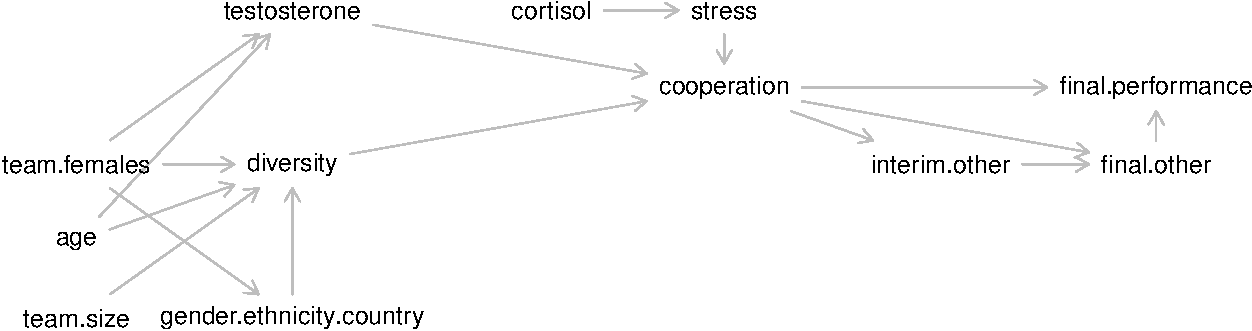
\includegraphics{19_10_02_hw5_q1_files/figure-latex/causal-1.pdf}
\caption{\label{fig:cause}Causal diagram illustrates hypothesized
relationships of experimental variables involved in relationship between
testosterone and final group performance.}
\end{figure}

\hypertarget{methods}{%
\subsection{Methods}\label{methods}}

\hypertarget{handling-missing-data}{%
\subsubsection{Handling missing data}\label{handling-missing-data}}

Before calculating additional team level statistics, we saw there were
\textless{}10 individuals with partly missing data. Since we are trying
to look at team level performance, we did not remove any individuals.
For these individuals, not everything was missing so we calculated group
average measurements, e.g.~average hormone measurements, from other
members.

From this we obtain a complete group level dataset where only
measurements in the `interim' variables are missing. Given that it's
unclear how the multiple interim measurements may relate to the final
score and they contain many missing values, we removed these variables.

\hypertarget{calculation-of-other-group-level-variables-from-individual-level-variables}{%
\subsubsection{Calculation of other group level variables from
individual level
variables}\label{calculation-of-other-group-level-variables-from-individual-level-variables}}

We are interested in doing our analysis at the group level therefore we
needed to aggregate the individual level data. To calculate group level
testosterone, cortisol and age we first averaged the corresponding
individual-level statistics, ignoring missing cases.

Additionally, we have calculated group diversity score as the number of
unique gender-ethnicity-country combinations present in the group.
Lastly we calculate proportion of females in the group as the number of
females divided by group size.

\hypertarget{exploratory-data-analysis-data-summary}{%
\subsection{Exploratory Data Analysis \& Data
Summary}\label{exploratory-data-analysis-data-summary}}

\hypertarget{distribution-of-hormone-levels-across-individuals-and-groups}{%
\subsubsection{Distribution of hormone levels across individuals and
groups}\label{distribution-of-hormone-levels-across-individuals-and-groups}}

It was clear when for both hormone levels that the log transformed
values were distributed with less skew across teams than the raw values
and have fewer outlier values. This is preferable so we chose like the
authors to use averaged log testosterone per group. Figure
\ref{fig:test} shows the distribtuions for testosterone but for cortisol
the difference is similar.

\begin{figure}
\centering
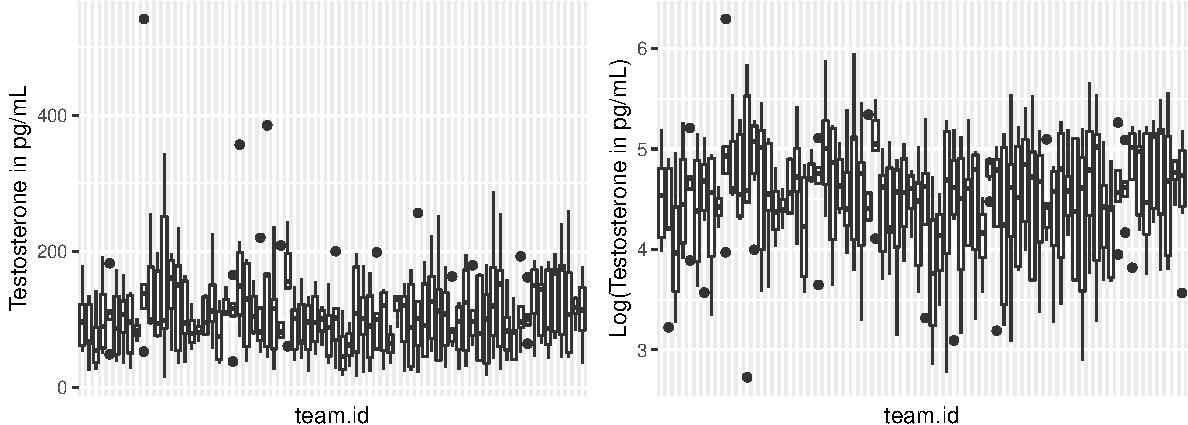
\includegraphics{19_10_02_hw5_q1_files/figure-latex/test-1.pdf}
\caption{\label{fig:test}Distributions of testosterone and log
testosterone levels in each team.}
\end{figure}

\hypertarget{univariate-and-pairwise-distributions-of-group-level-variables}{%
\subsubsection{Univariate and pairwise distributions of group level
variables}\label{univariate-and-pairwise-distributions-of-group-level-variables}}

The univariate distributions of the group level variables is given
across the diagonal in Figure \ref{fig:pairs}. We see that in
particular, our diversity score appears bimodal. Although our score is
calculated differently, (Akinola et al. 2018) classified diversity score
into two bins in their faultline analysis suggesting that our diversity
score may behave similarly.

In the same figure we have the pairwise comparisons of the important
variables as well. In the upper diagonal, the Pearson correlation
coefficients (upper right half) between important variables are
described with their significance.

Looking at this figure, we can make the following observations about the
key variables:

\begin{itemize}
\tightlist
\item
  We do not need to remove variables based on collinearity.
\item
  performance appears correlated with proportion of females and
  testosterone.
\item
  In addition to performance, testosterone appears significantly
  correlated with cortisol, average age, proportion of females, time of
  day, and team size.
\item
  diversity score appears significantly correlated with team size.
\end{itemize}

Based on this we believe that in addition to final.performance,
avg.log.testosterone, avg.log.cortisol and diversity.score we should
consider whether to incorporate the four additional variables
proportion.female, avg.age/age.variance, time.of.day, and team.size in
our models.

\begin{figure}
\centering
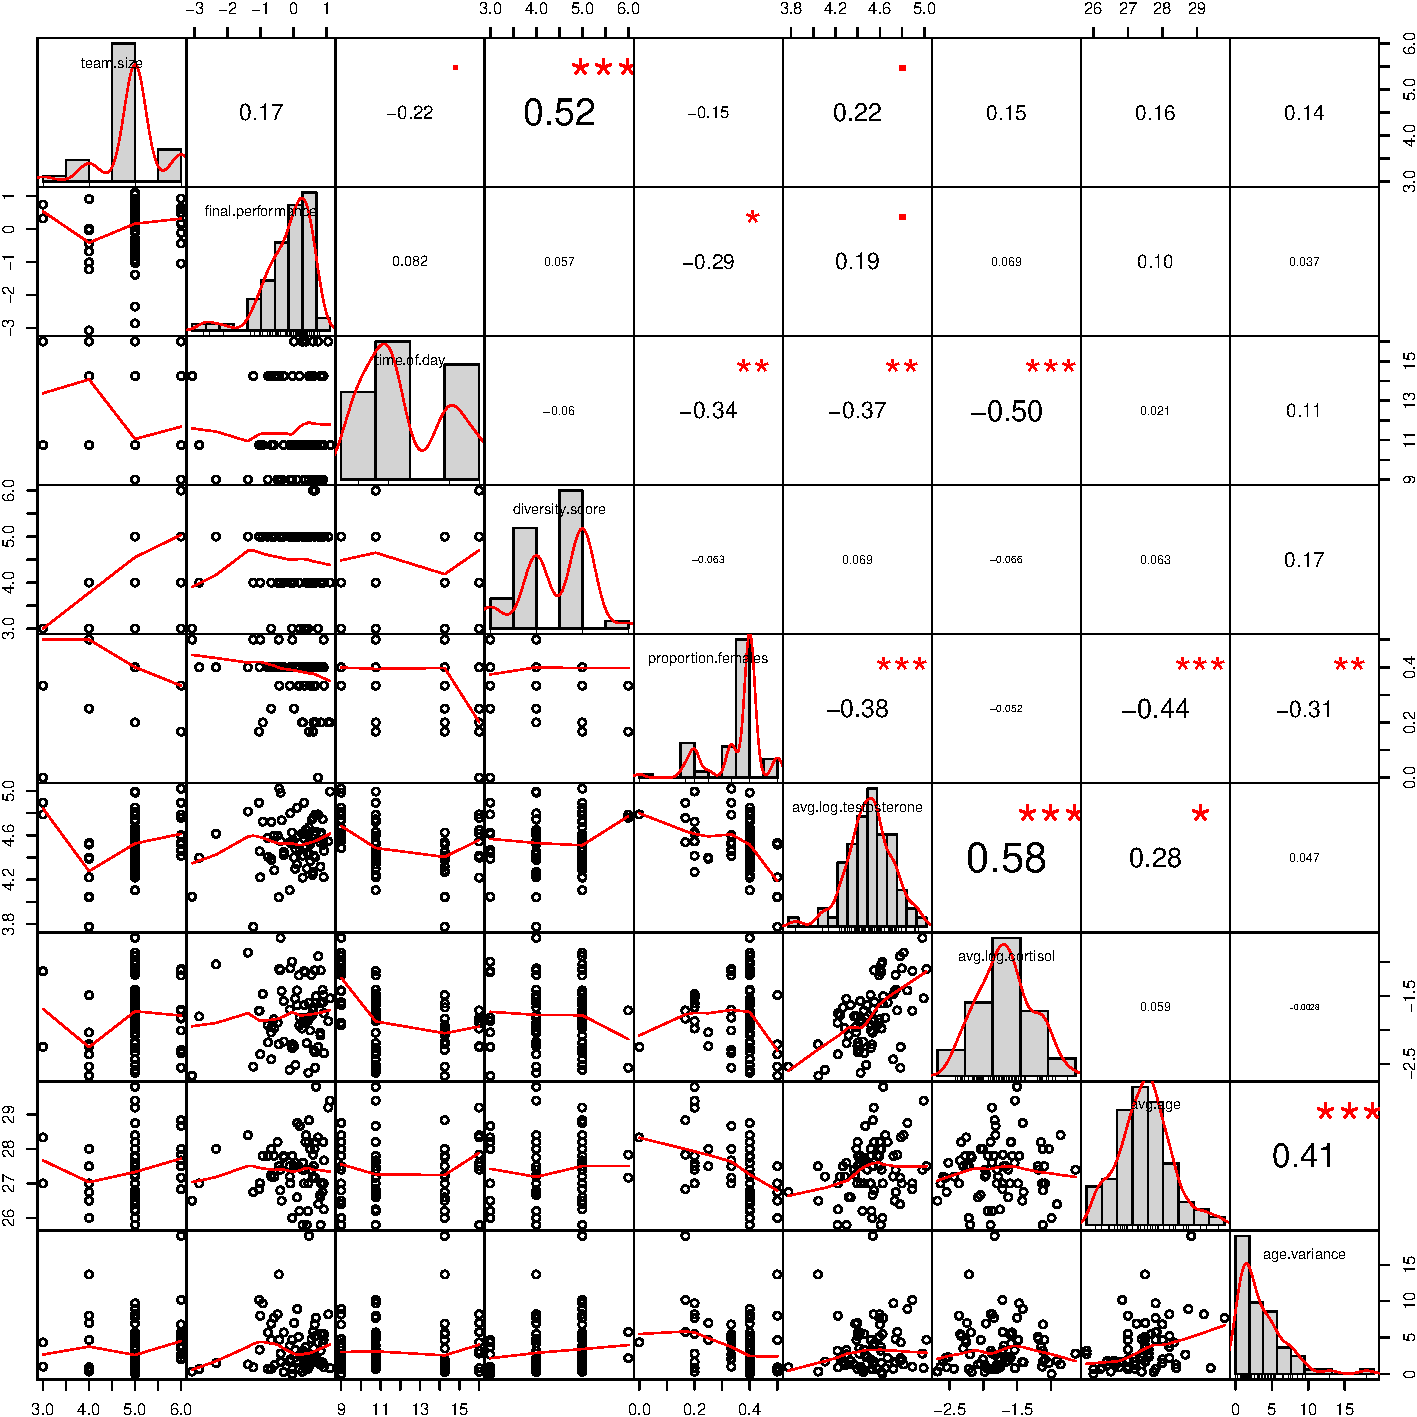
\includegraphics{19_10_02_hw5_q1_files/figure-latex/dists-1.pdf}
\caption{\label{fig:pairs}Pairwise correlations of important variables
including their Pearson correlation coefficient. Significant
correlations are marked by the corresponding number of astericks.}
\end{figure}

\hypertarget{results}{%
\subsection{Results}\label{results}}

The results discussed by the original study (Akinola et al. 2018)
include that:

\begin{itemize}
\tightlist
\item
  considered in isolation, group diversity and testosterone are not
  significantly correlated with performance.
\item
  when group diversity was low, group testosterone significantly
  positively predicted performance at p \textless{} .01
\item
  when group diversity was relatively high, group testosterone
  significantly negatively predicted performance p \textless{}0.01
\end{itemize}

\hypertarget{diversity-score-and-testosterone-do-not-individually-significantly-predict-performance}{%
\subsubsection{Diversity score and testosterone do not individually
significantly predict
performance}\label{diversity-score-and-testosterone-do-not-individually-significantly-predict-performance}}

To start we want to check the simplest assumptions from (Akinola et al.
2018) that diversity score and testosterone do not significantly predict
performance on their own. We use the F-test to compare this null
hypothesis to the alternative hypothesis where the model only contains
an intercept term (Table \ref{fig:model}).

\begin{table}[!htbp] \centering 
  \caption{} 
  \label{} 
\begin{tabular}{@{\extracolsep{5pt}}lcc} 
\\[-1.8ex]\hline 
\hline \\[-1.8ex] 
 & \multicolumn{2}{c}{\textit{Dependent variable:}} \\ 
\cline{2-3} 
\\[-1.8ex] & \multicolumn{2}{c}{final.performance} \\ 
\\[-1.8ex] & (1) & (2)\\ 
\hline \\[-1.8ex] 
 Constant & $-$3.181 & $-$0.292 \\ 
  & (1.910) & (0.614) \\ 
  & & \\ 
 avg.log.testosterone & 0.703$^{*}$ &  \\ 
  & (0.422) &  \\ 
  & & \\ 
 diversity.score &  & 0.066 \\ 
  &  & (0.136) \\ 
  & & \\ 
\hline \\[-1.8ex] 
Observations & 74 & 74 \\ 
R$^{2}$ & 0.037 & 0.003 \\ 
Adjusted R$^{2}$ & 0.024 & $-$0.011 \\ 
Residual Std. Error (df = 72) & 0.828 & 0.843 \\ 
F Statistic (df = 1; 72) & 2.783$^{*}$ & 0.232 \\ 
\hline 
\hline \\[-1.8ex] 
\textit{Note:}  & \multicolumn{2}{r}{$^{*}$p$<$0.1; $^{**}$p$<$0.05; $^{***}$p$<$0.01} \\ 
\end{tabular} 
\end{table}

For these simple models, the coefficient of diversity score (0.066) and
average log testosterone (0.703) are not large in magnitude or
significant (p \textgreater{}0.05) indicating that we do not reject the
null hypothesis. This agrees with what the authors found.

\hypertarget{group-diversity-on-relationship-between-testosterone-and-performance}{%
\subsubsection{Group diversity on relationship between testosterone and
performance}\label{group-diversity-on-relationship-between-testosterone-and-performance}}

Next we fit a model to examine whether including an interaction between
them could predict performance.

\begin{longtable}[]{@{}lr@{}}
\toprule
& x\tabularnewline
\midrule
\endhead
(Intercept) & -48.112\tabularnewline
avg.log.testosterone & 10.274\tabularnewline
diversity.score & 10.189\tabularnewline
team.size & 0.353\tabularnewline
avg.log.testosterone:diversity.score & -2.258\tabularnewline
\bottomrule
\end{longtable}

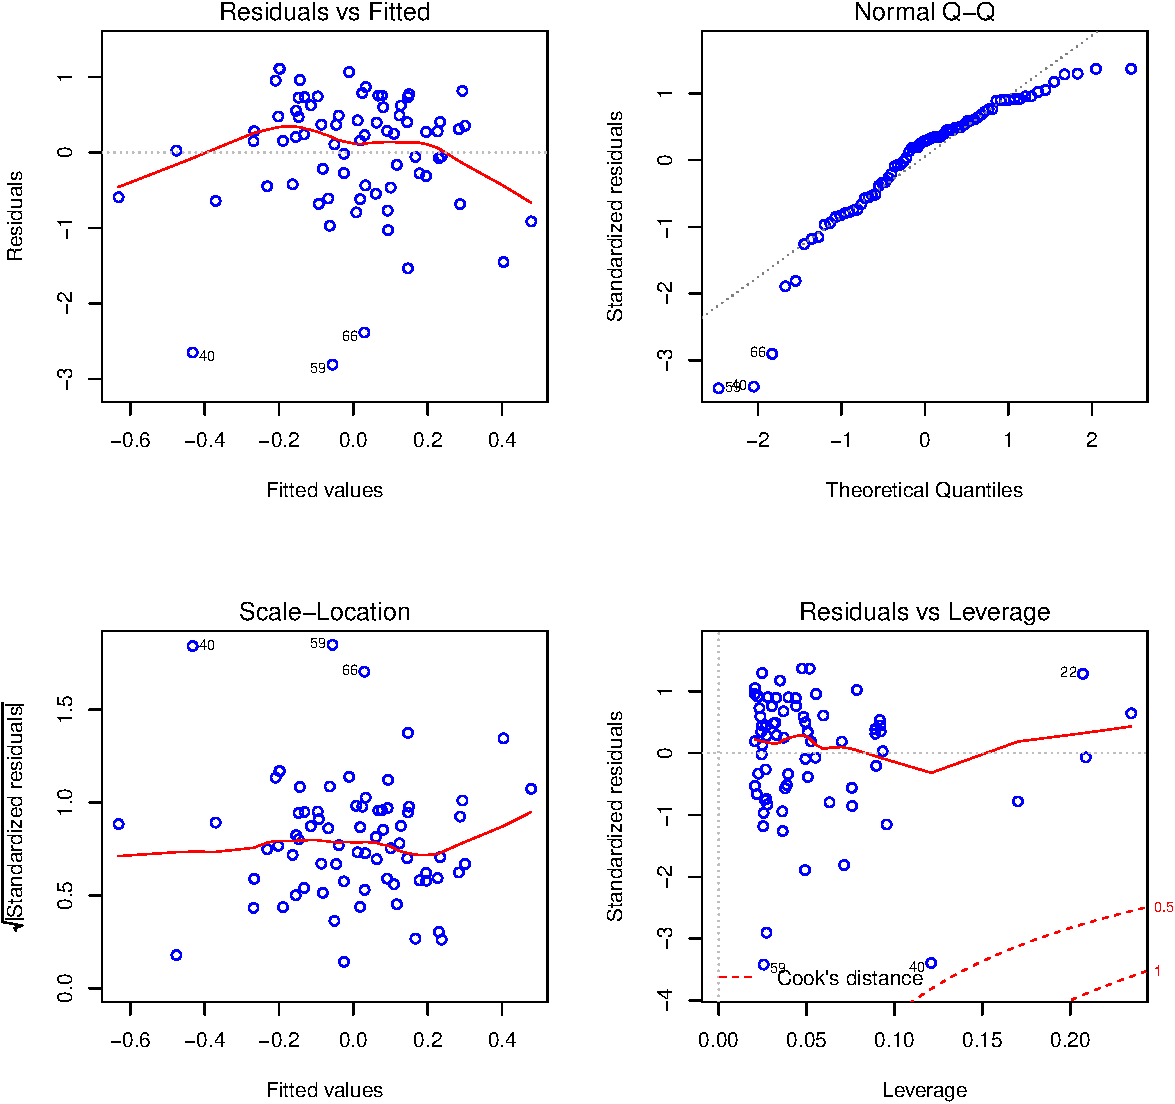
\includegraphics{19_10_02_hw5_q1_files/figure-latex/test_model-1.pdf} We
found a significant positive effect of testosterone on performance when
controlling for diversity score and team size (coefficient = 10.2743, p
\textless{} 0.001). Further we find a significant positive effect of
diversity score on performance when controlling for testosterone, team
size and their interaction (coefficient = 10.1889, p \textless{} 0.001).
The interaction term has a negative coefficient. This suggests that
whereas each of testosterone and diversity aids performance, their
interaction works against these effects. Our results are in line with
those of the original study.

\hypertarget{q5-effect-of-cortisol-on-relationship-between-diversity-and-performance}{%
\subsubsection{Q5: Effect of cortisol on relationship between diversity
and
performance}\label{q5-effect-of-cortisol-on-relationship-between-diversity-and-performance}}

Figure \ref{fig:pairs} suggested a weakly linear relationship between
cortisol and performance (pearson correlation coefficient of )

Accordingly, when we fit the very simplest model of final.performance
\textasciitilde{} avg.log.cortisol, we find a positive (0.1217) but not
significant (p-value 0.56) coefficient as our scatterplots above may
suggest.

\hypertarget{model-with-interaction-of-cortisol-and-diversity-score}{%
\subsubsection{Model with interaction of cortisol and diversity
score}\label{model-with-interaction-of-cortisol-and-diversity-score}}

Next, we tested whether cortisol levels could change the relationship
between diversity score and performance with a model containing each of
these variables and their three way interaction. Again we are
controlling for team size by including it as a term in the model.

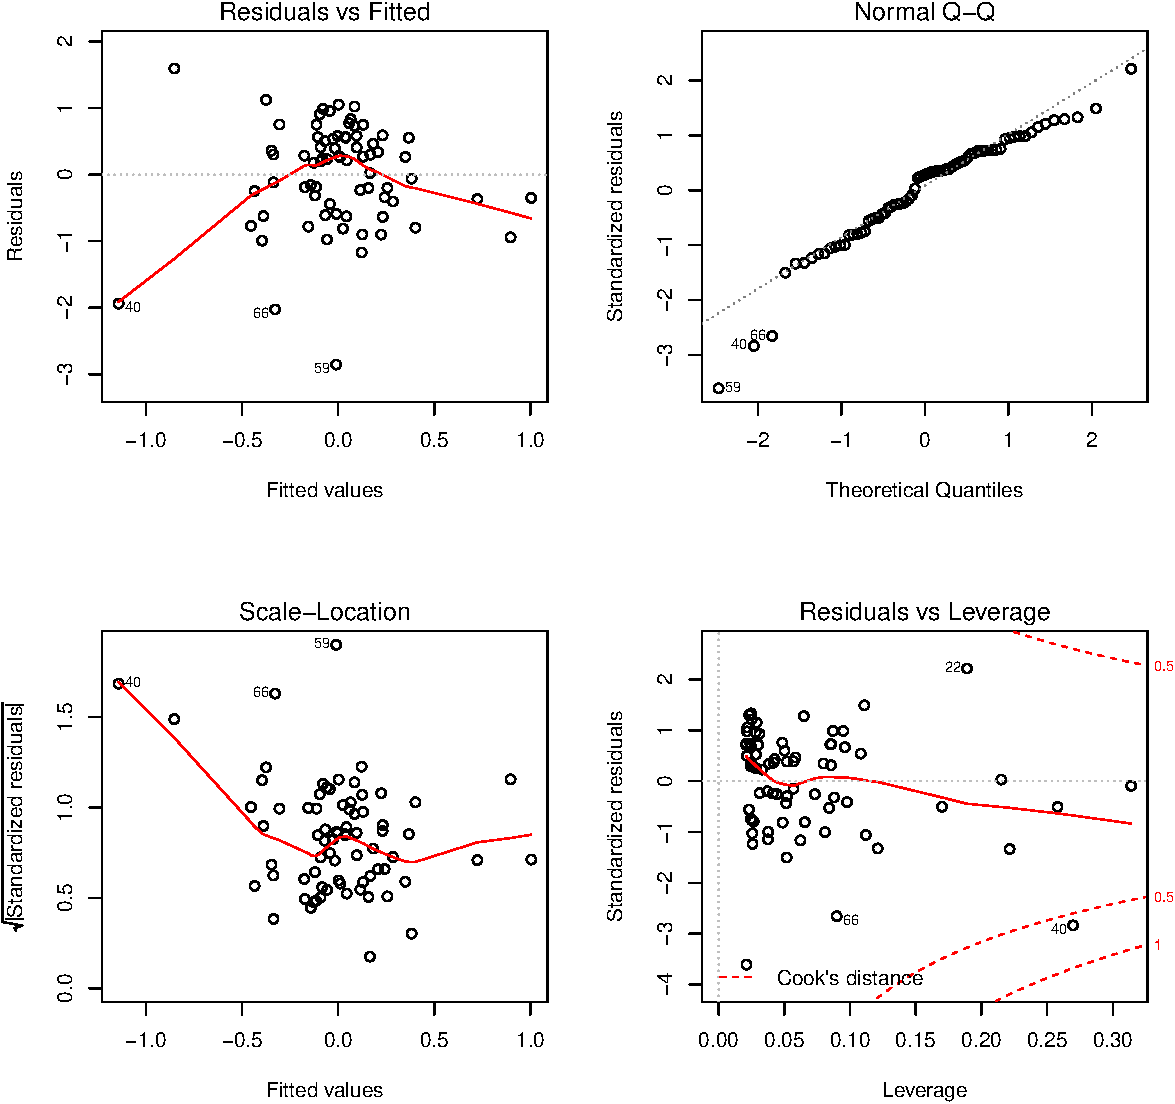
\includegraphics{19_10_02_hw5_q1_files/figure-latex/stress-1.pdf} We
found that stress seems to positively impact performance (coefficient of
3.348 units, p \textless{} 0.01) when controlling for diversity score,
team size and the interaction between cortisol and diversity score.
However, the diversity score is estimated here to have a negative effect
on performance (coefficient of -6.8455 units, p \textless{} 0.05).
Furthermore the interaction term also has a weak negative effect
(coefficient of -0.7483 units, p \textless{} 0.05).

This suggests stressed groups have better performance and stress changes
the effect of diversity to negatively impact performance.

\hypertarget{conclusion}{%
\subsubsection{Conclusion}\label{conclusion}}

Here we have analyzed demographic data and hormone measurements from
groups of MBA students performing a competetive project, previously
published by (Akinola et al. 2018). We sought to investigate the
authors' hypothesis that group diversity has a testosterone-dependent
effect on group performance and also to check whether cortisol levels
had an effect on this relationship.

By building linear models of performance and testing the significance of
the terms with an F-test, we have shown that although testosterone and
diversity score alone do not predict performance, when they are both
included in the model interaction between diversity and testosterone has
a significant negative effect on performance (p \textless{} 0.01)
implying that high diversity and high testosterone are antagonizing
factors. Although stressed groups did not have significantly different
performance, we also found that when controlling for diversity cortisol
has similar effects. The interaction between cortisol and diversity also
has a significant negative effect on performance (p \textless{} 0.05)
implying that higher diversity and higher cortisol counteract each
other. When looking at both hormone measurements simultaneously with
diversity score, surprisingly we found that when accounting for
cortisol, testosterone levels do not seem to have a significant effect
on performance. Rather only the interaction of cortisol and testosterone
together has a slight negative effect on performance (p \textless{}
0.01). However, the model we tested containing both hormones has a lower
adjusted R squared than the model containing just testosterone. Overall,
we do find that diversity is beneficial for performance, in the presence
of low group-level testosterone. Additionally this analysis suggests
that perhaps, stress has a role in group performance as well.

Although we had some similar findings to the original study when
examining diversity and testosterone, our results may not be directly
comparable because of some differences in our methodology. Most
prominently, (Akinola et al. 2018) have used a faultline analysis to
evaluate diversity whereas we have constructed a diversity score. As
well, we have not included some of the variables that are present in the
models which they tested e.g.~proportion of females. We chose to discard
these variables based upon our EDA and our reasoning about the
relationship between variables collected in the study. Lastly we cannot
compare our findings about cortisol because this was not discussed in
depth in their original analysis.

\hypertarget{bibliography}{%
\section*{Bibliography}\label{bibliography}}
\addcontentsline{toc}{section}{Bibliography}

\hypertarget{refs}{}
\leavevmode\hypertarget{ref-Akinola2018}{}%
Akinola, Modupe, Elizabeth Page-Gould, Pranjal H. Mehta, and Zaijia Liu.
2018. ``Hormone-Diversity Fit: Collective Testosterone Moderates the
Effect of Diversity on Group Performance.'' \emph{Psychological Science}
29 (6):859--67. \url{https://doi.org/10.1177/0956797617744282}.

\leavevmode\hypertarget{ref-Kelsey2014}{}%
Kelsey, Thomas W., Lucy Q. Li, Rod T. Mitchell, Ashley Whelan, Richard
A. Anderson, and W. Hamish B. Wallace. 2014. ``A Validated Age-Related
Normative Model for Male Total Testosterone Shows Increasing Variance
but No Decline after Age 40 Years.'' Edited by Bin He. \emph{PLoS ONE} 9
(10):e109346. \url{https://doi.org/10.1371/journal.pone.0109346}.

\leavevmode\hypertarget{ref-vanK}{}%
Knippenberg, Daan van, and Michaéla C. Schippers. 2007. ``Work Group
Diversity.'' \emph{Annual Review of Psychology} 58 (1):515--41.
\url{https://doi.org/10.1146/annurev.psych.58.110405.085546}.

\leavevmode\hypertarget{ref-matsu}{}%
Matsuzaka, Hisashi, Hitoshi Maeshima, Sayaka Kida, Hirofumi Kurita,
Takahisa Shimano, Yoshiyuki Nakano, Hajime Baba, Toshihito Suzuki, and
Heii Arai. 2013. ``Gender Differences in Serum Testosterone and Cortisol
in Patients with Major Depressive Disorder Compared with Controls.''
\emph{The International Journal of Psychiatry in Medicine} 46
(2):203--21. \url{https://doi.org/10.2190/PM.46.2.g}.

\leavevmode\hypertarget{ref-MEHTA2015163}{}%
Mehta, Pranjal H, and Smrithi Prasad. 2015. ``The Dual-Hormone
Hypothesis: A Brief Review and Future Research Agenda.'' \emph{Current
Opinion in Behavioral Sciences} 3:163--68.
\url{https://doi.org/https://doi.org/10.1016/j.cobeha.2015.04.008}.


\end{document}
